\documentclass{ximera}

%\addPrintStyle{..}

\begin{document}
	\author{Bart Lambregs}
	\xmtitle{De horizontale worp}{}
    \xmsource\xmuitleg

We bekijken een voorbeeld van een tweedimensionale beweging. Wanneer een object horizontaal met een bepaalde beginsnelheid wordt gekatapulteerd, noemen we die beweging een horizontale worp. Wij beschouwen de worp in het luchtledige.
\begin{image}
	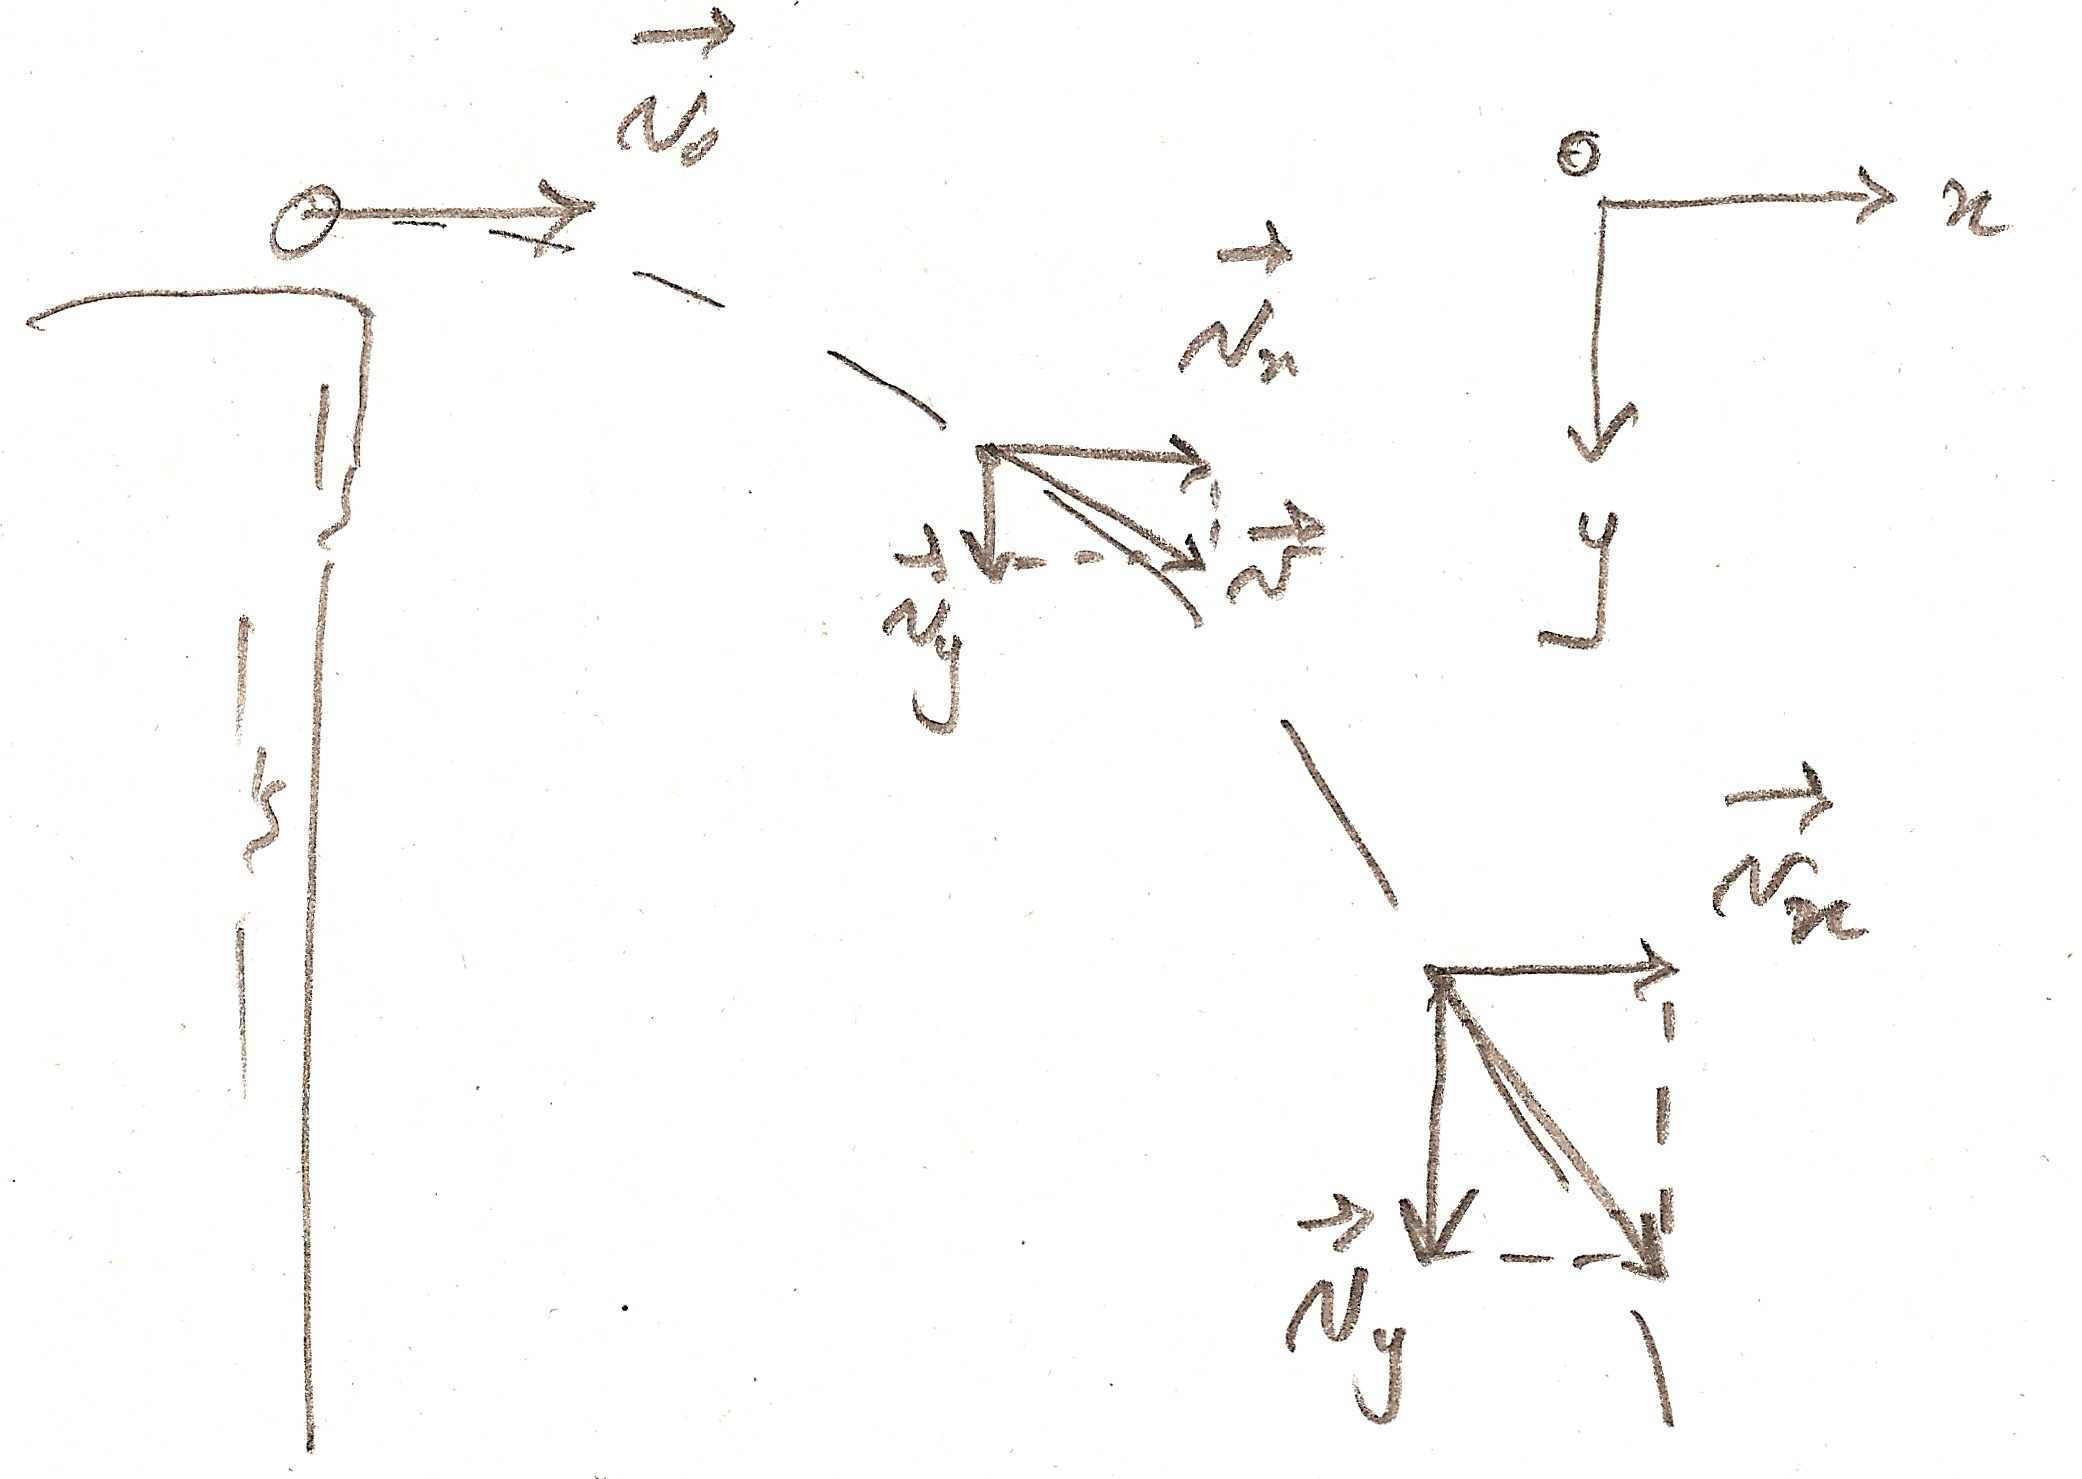
\includegraphics[width=0.6\textwidth]{horizontaleworp_tekening}
\end{image}
\captionof{figure}{De snelheid in horizontale richting verandert niet, die in de verticale richting neemt lineair toe in de tijd}

In de beschrijving kunnen we de $x$-as horizontaal en de $y$-as verticaal naar beneden nemen. Omdat er volgens de $x$-as geen versnelling is het lichaam volgens de $y$-as valt met de valversnelling $g$, kunnen we de formules voor een ERB en een EVRB op de afzonderlijke assen toepassen en zo de volledige beweging beschrijven.
\begin{equation*}
	\left\{
	\begin{array}{l}
	a_x=0\\
	a_y=g
	\end{array}
	\right.
	\Rightarrow
	\left\{
	\begin{array}{l}
	v_x=v_0\\
	v_y=gt
	\end{array}
	\right.
	\Rightarrow
	\left\{
	\begin{array}{l}
	x=v_0t\\
	y=\frac{1}{2}gt^2
	\end{array}
	\right.
\end{equation*}
De baanvergelijking vinden we zoals eerder vermeld, door $t$ in functie van $x$ te schrijven $x=v_0t\Leftrightarrow t=\frac{x}{v_0}$ en dit in $y(t)$ te substitueren:
\begin{eqnarray*}
	y=\frac{1}{2}gt^2=\frac{1}{2}g\left(\frac{x}{v_0}\right)^2=\frac{g}{2v_0^2}x^2
\end{eqnarray*}
De baan is dus een parabool.

\begin{example}
	Een vliegtuig vliegt met een snelheid van \SI{450}{km/h} op een hoogte van \SI{920}{m}.
	\begin{enumerate}
		\item Hoever voor het doel moeten de voedselpakketten gelost worden om op het doel terecht te komen?
		\item Hoeveel tijd hebben de pakketten nodig om het doel te bereiken?
	\end{enumerate}
	De afstand waarover de voedselpakketten in horizontale richting zijn vooruit gegaan, kunnen we vinden met de baanvergelijking. We weten namelijk hoever de pakketten naar beneden zijn gevallen en wat hun beginsnelheid is:
	\begin{eqnarray*}
		y&=&\frac{g}{2v_0^2}x^2\\
		&\Downarrow&\\
		x&=&v_0\sqrt{\frac{2y}{g}}=\SI{1712}{m}
	\end{eqnarray*}
	De valtijd voor de pakketten vinden we o.a. door naar de verticale valbeweging te kijken. Deze gebeurt onafhankelijk van wat er in de horizontale richting gebeurt, zodat:
	\begin{eqnarray*}
		y&=&\frac{1}{2}gt^2\\
		&\Downarrow&\\
		t&=&\sqrt{\frac{2y}{g}}=\SI{13,7}{s}
	\end{eqnarray*}
\end{example}
	
\end{document}
